\begin{enumerate}
    \item  Bellmam Equation $$v(k_t)= max_{k_{t+1}} \frac{(k_t^\theta -k_{t+1}+(1-\delta)k_t)^{1-\sigma}-1}{1-\sigma}+\beta v(k_{t+1})$$\\
    FOC: please note $x_t=k_t, y_t=k_{t+1}$ please also note that $x_{s+1}=G(x_s,y_s)$
    
    $$\frac{\partial v(k_t)}{\partial k_{t+1}}=-( -k_{t+1} + (1-\delta)*k_t +k_t^\theta)^{-\sigma}
   +\beta v'(G(x_t,y_t))*G_{x_t}(x_{t+1},y_{t+1})$$
   non zero steady state 
   $$$$
   \item. 
   \item .
   \newline
   \begin{figure}[H]
       \centering
       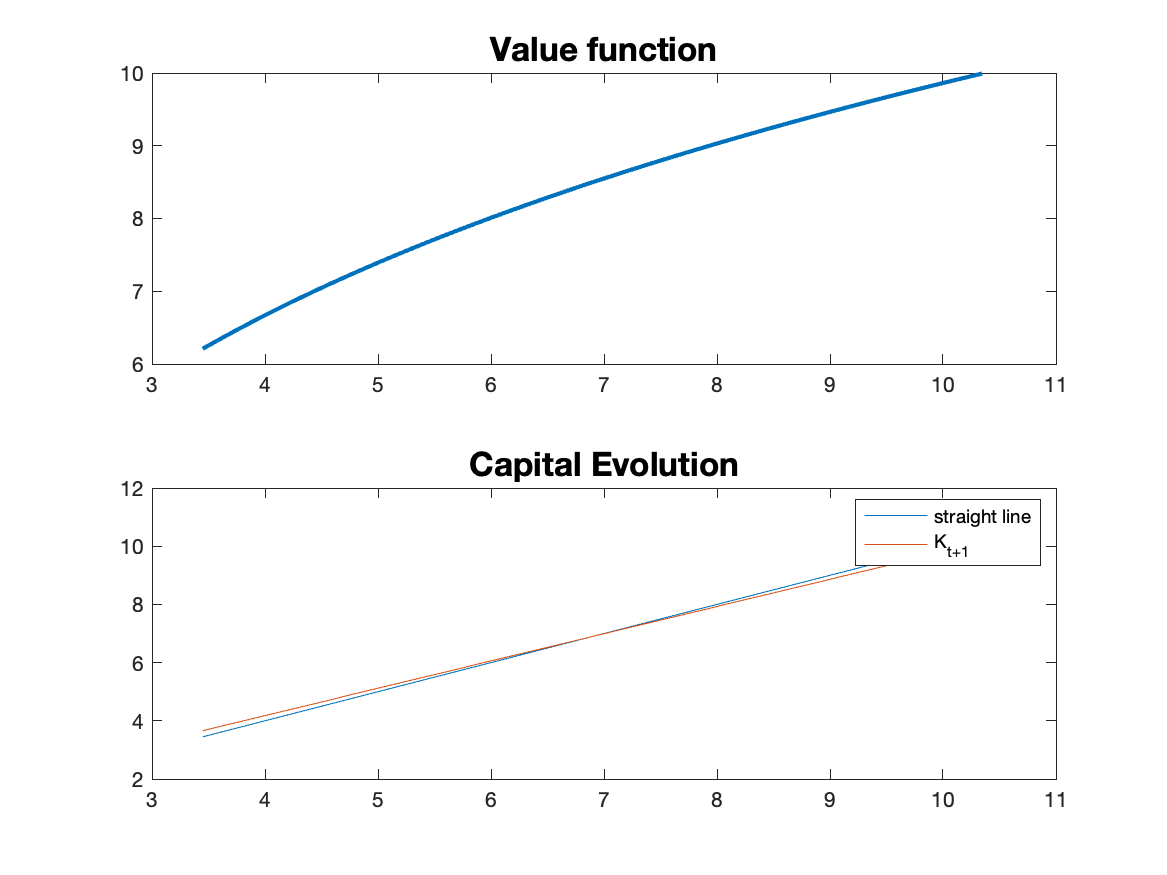
\includegraphics[width = .7\linewidth]{HW3/pics/HW3_Q2_figure.png}
       \caption{The steady state equilibrium would be stable as the $k_{t+1}$ function is above the 45 degree line before the steady state and below the 45 degree line after the steady state}
       \label{fig:HW3_2c}
   \end{figure}
   \item see above
   \item 
   \begin{figure}[H]
       \centering
       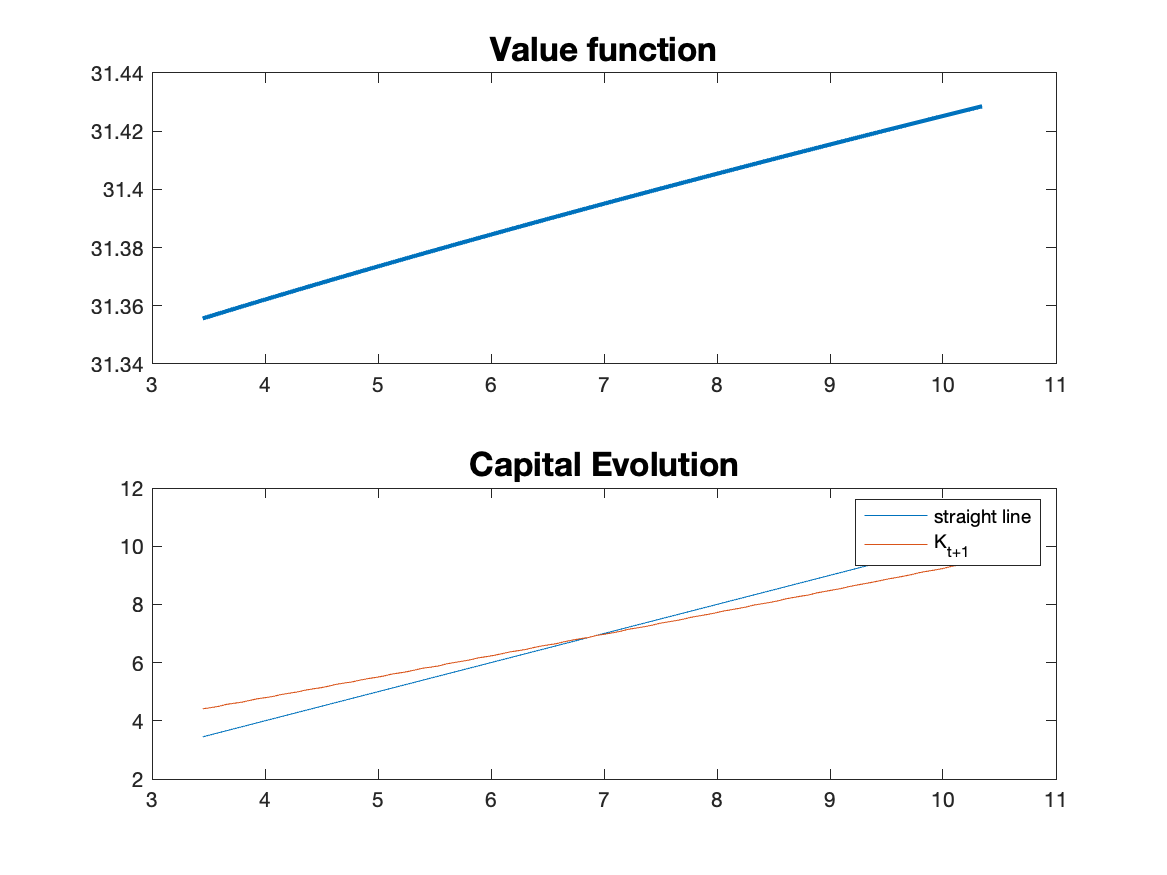
\includegraphics[width = .7\linewidth]{HW3/pics/HW3_Q2_e_figure.png}
       \caption{Similar to part c, the steady state equilibrium would be stable. The main difference is the slow of the $K_{t+1}$ line. This time the line is much less steep than the solution in part c.}
       \label{fig:HW3_2e}
   \end{figure}
\end{enumerate}